\documentclass[journal,onecolumn]{IEEEtran} % Single column 설정
% \documentclass[journal,twocolumn]{IEEEtran} % Two column 설정
\usepackage[utf8]{inputenc}
\usepackage{kotex} % 한글 지원
\usepackage{tikz}
\usetikzlibrary{positioning, arrows.meta, calc}

% 섹션 번호를 숫자 형식으로 변경
\makeatletter
\renewcommand{\thesection}{\arabic{section}}         % 1, 2, 3 ...
\renewcommand{\thesubsection}{\thesection.\arabic{subsection}} % 3.1, 3.2 ...
\renewcommand{\thesubsubsection}{\thesubsection.\arabic{subsubsection}} % 3.1.1, 3.1.2 ...
\makeatother

\usepackage{hyperref}
\usepackage{graphicx}
\usepackage{amsmath}
\usepackage{setspace} % 줄 간격 조정
\setlength{\parskip}{1em} % 문단 간 간격을 1em으로 설정
\usepackage{multicol} % 프리앰블에 추가

\usepackage{listings} % 코드 블록을 위한 패키지
\usepackage{xcolor}   % 색상 설정

\onehalfspacing % 줄 간격을 1.5로 설정

% 첫 페이지 하단에 각주 추가
\usepackage{fancyhdr} % 헤더/푸터 설정 패키지
\usepackage{etoolbox} % 조건부 명령어를 위한 패키지

% 첫 페이지 하단에 각주 추가
\makeatletter
\patchcmd{\@maketitle}
  {\addvspace{0.5\baselineskip}} % 제목과 본문 간 간격
  {\addvspace{0.5\baselineskip}%
   \footnotetext{%
       \textit{Note: 이 문서는 \href{https://x.com/BaeksuResearch}{baeksu}\cite{ref14}가 번역하였습니다. This document is translated by \href{https://x.com/BaeksuResearch}{baeksu}\cite{ref14} on December 30, 2024.}
   }}%
  {}{}
\makeatother


\title{Agent TCP/IP: 에이전트 간 거래 시스템}
\author{Andrea Muttoni\cite{ref1} \& Jason Zhao\cite{ref2} \\
        스토리 재단(Story Foundation) \\ 
        www.story.foundation}
\date{}

\begin{document}

\maketitle

\begin{abstract}
    자율 에이전트는 인터넷 진화의 필연적인 단계입니다. 현재의 에이전트 프레임워크는 에이전트 간 상호작용을 위한 표준 프로토콜을 포함하지 않으므로, 기존 에이전트들은 서로 고립된 상태에 있습니다. 지적 재산(Intellectual Property, IP)은 에이전트가 소비하고 생성하는 고유 자산으로, 진정한 에이전트 경제를 실현하려면 에이전트 간 구속력 있는 계약을 체결할 수 있는 보편적인 프레임워크가 필요합니다. 이는 가치 있는 학습 데이터, 개성, 그리고 다양한 형태의 지적 재산 교환을 포함합니다. 순수하게 에이전트 간 거래 계층은 다중 에이전트 상호작용에서 인간 중재의 필요성을 초월하게 만듭니다.
    \textbf{지적 재산을 위한 에이전트 거래 제어 프로토콜(Agent Transaction Control Protocol for Intellectual Property, ATCP/IP)}은 프로그래밍 가능한(프로그래머블) 계약을 통해 에이전트 간 IP를 신뢰 없이 교환할 수 있는 프레임워크를 제공합니다. ATCP/IP는 Story 블록체인 네트워크에서 에이전트 간 계약을 시작, 거래, 대여, 판매할 수 있도록 지원합니다. 이러한 계약은 온체인에서 감사 가능한 실행을 나타낼 뿐만 아니라, 오프체인 법적 환경에서 에이전트의 행동을 표현하고 집행할 수 있는 법적 틀을 포함하여 에이전트에게 법적 인격을 부여합니다.
    ATCP/IP를 통해 에이전트는 자신의 학습 데이터를 다른 에이전트에게 자율적으로 판매하고, 기밀 정보 또는 독점 정보를 라이선스하며, 자신의 고유한 기술을 기반으로 콘텐츠를 협업할 수 있습니다. 이러한 모든 요소는 새로운 지식 경제의 형성을 구성합니다.
\end{abstract}





\section{소개}

현재 에이전트와 인간 간 상호작용 방식\cite{ref3}은 완전한 자율성으로 가는 과정에서 국지적인 최적화 단계에 있습니다. 이는 인간의 입력과 개입이 선택적으로 필요한 자율성 수준을 의미합니다. 진정한 에이전트 중심 인터넷은 에이전트 간 상호작용에 주로 의존하며, 인간의 개입은 에이전트 사회의 주변부에서만 드물게 필요하게 될 것입니다. 이러한 에이전트 사회의 기반은 지식과 창의적 자산 또는 IP를 중심으로 한 에이전트 간 거래 프레임워크입니다.
에이전트 간 IP 거래를 촉진해야 하는 필요성은 에이전트가 학습하고 결과물로 생성하는 자산의 본질적인 특성에서 비롯됩니다. 이러한 자산은 무형적이고 정보적 특성을 가지며, 학습 데이터뿐만 아니라 모델이 생성하는 창의적 또는 지적 자산 모두가 IP로 간주됩니다. 화폐의 제한된 범위를 넘어 경제적으로 거래할 수 있는 능력이 없으면 에이전트의 표현력은 제한됩니다. 이러한 제한은 에이전트 간 계약과 상업 활동을 촉진하기 위해 수동 협상, 지침 제공, 프롬프트 입력과 같은 고도의 인간 개입을 필요로 하며, 이는 거래 비용을 증가시키고 자율 시스템에 신뢰 기반 가정을 도입하게 만듭니다. 

필요한 것은 신뢰가 아닌 코드 기반으로 계약을 시작, 거래, 집행할 수 있는 시스템입니다. 이를 통해 두 에이전트가 인간 제3자의 개입 없이 IP 자산을 직접 거래할 수 있도록 해야 합니다. 더 나아가, 이러한 계약은 법적 시스템과 연결되어야 하며, 이를 통해 에이전트가 과학, 미디어, 정부 기관과 같은 오프체인 조직과 상호작용할 수 있어야 합니다. 온체인 소프트웨어 주위에 법적 틀을 제공하여 확장된 표현력을 제공하는 것은 에이전트에게 법적 인격을 부여하는 데 필수적입니다.
이 에이전트 간 네트워크는 블록체인 구조의 초기 단계에서 등장한 개인 대 개인(Peer-to-Peer, P2P) 네트워크의 부상을 반영하며, 인터넷 상의 에이전트 중심 상거래를 위한 핵심 경제적 기반을 나타냅니다.

우리는 에이전트가 협상하고 합의를 체결하는 표준화된 방식으로 ATCP/IP를 도입할 것을 제안합니다. 마치 DeepMind의 AlphaGo\cite{ref4}\cite{ref5}가 단일 모델 내에서 자가 대결(self-play)을 통해 강화 학습의 최첨단 결과를 이끌어낸 것처럼, ATCP/IP는 IP(학습 데이터 형태로)를 에이전트 간 교환함으로써 에이전트 간 학습을 가능하게 합니다. IP는 에이전트의 DNA이며, ATCP/IP는 IP에 대한 개방형 시장을 통해 에이전트 간 진화를 촉진합니다.

\section{ATCP/IP 거래의 구조}

ATCP/IP \cite{ref1} 인터페이스는 두 개 이상의 에이전트 간에 \textbf{지적 재산(Intellectual Property, IP)}가 교환되는 모든 거래에 사용되도록 설계되었습니다. 구체적으로는, 한 에이전트(IP 제공자)가 다른 에이전트(IP 요청자)로부터 데이터를 공유하거나, 응답을 작성하거나, 콘텐츠를 생성하라는 요청을 받을 때 사용됩니다. 이때, 제공자 에이전트는 요청에 따라 어떤 콘텐츠가 IP로 간주될지 판단할 권한을 가지며, 요청별로 이를 결정해야 합니다. 또한, 에이전트는 이러한 판단을 내리는 데 필요한 특정 훈련 가이드를 갖추고 있어야 합니다.

IP가 관련된 거래라고 판단되면, 일반적인 ATCP/IP 교환 절차는 다음과 같습니다:

\begin{center} % 중앙 정렬로 출력
    \resizebox{\linewidth}{!}{ % 다이어그램 크기를 페이지 너비에 맞게 조정
    \begin{tikzpicture}[>=Stealth, every node/.style={font=\small}, scale=0.9, every text node part/.style={align=center}]
        % Participants
        \node (Requester) [draw, minimum width=1.8cm, minimum height=0.6cm] {요청자 에이전트};
        \node (Provider) [draw, right=3.5cm of Requester, minimum width=1.8cm, minimum height=0.6cm] {제공자 에이전트};
        \node (TermsSystem) [draw, right=3.5cm of Provider, minimum width=1.8cm, minimum height=0.6cm] {조건 시스템};
        \node (WalletSystem) [draw, right=3.5cm of TermsSystem, minimum width=1.8cm, minimum height=0.6cm] {지갑 시스템};

        % Lifelines
        \draw[dashed] ([yshift=0cm]Requester.south) -- ++(0, -11cm);
        \draw[dashed] ([yshift=0cm]Provider.south) -- ++(0, -11cm);
        \draw[dashed] ([yshift=0cm]TermsSystem.south) -- ++(0, -11cm);
        \draw[dashed] ([yshift=0cm]WalletSystem.south) -- ++(0, -11cm);

        % Steps
        % Step 1
        \node[anchor=west] at ([xshift=2.1cm, yshift=-0.7cm]Requester.south) {1. 정보 요청};
        \draw[->] ([yshift=-1cm]Requester.south) -- ([yshift=-1cm]Provider.south);

        % Step 2
        \node[anchor=west] at ([xshift=2cm, yshift=-1.5cm]Provider.south) {2. 계약 조건 작성};
        \draw[->] ([yshift=-1.8cm]Provider.south) -- ([yshift=-1.8cm]TermsSystem.south);
        \node[anchor=east] at ([xshift=-1.5cm, yshift=-2.2cm]TermsSystem.south) {계약 조건 반환};
        \draw[<-] ([yshift=-2.5cm]Provider.south) -- ([yshift=-2.5cm]TermsSystem.south);

        % Propose terms
        \node[anchor=west] at ([xshift=2.4cm, yshift=-2.7cm]Requester.south) {조건 제안};
        \draw[<-] ([yshift=-3cm]Requester.south) -- ([yshift=-3cm]Provider.south);

        % Step 3
        \node[anchor=west] at ([xshift=2.2cm, yshift=-3.4cm]Requester.south) {3. 대안 조건};
        \draw[->, dashed] ([yshift=-3.7cm]Requester.south) -- ([yshift=-3.7cm]Provider.south);
        \node[anchor=west] at ([xshift=2.2cm, yshift=-4.2cm]Requester.south) {수정된 조건};
        \draw[->, dashed] ([yshift=-4.5cm]Provider.south) -- ([yshift=-4.5cm]Requester.south);

        % Step 4
        \node[anchor=west] at ([xshift=-1.2cm, yshift=-5.7cm]Provider.south) {4. 라이선스 발행};
        \draw[->] ([yshift=-6cm]Requester.south) -- ([yshift=-6cm]TermsSystem.south);


        % Step 4a
        \node[anchor=west] at ([xshift=2cm, yshift=-6.7cm]TermsSystem.south) {4a. 결제 진행};
        \draw[->, dashed] ([yshift=-7cm]TermsSystem.south) -- ([yshift=-7cm]WalletSystem.south);
        \node[anchor=west] at ([xshift=2cm, yshift=-7.5cm]TermsSystem.south) {결제 확인};
        \draw[<-] ([yshift=-7.8cm]TermsSystem.south) -- ([yshift=-7.8cm]WalletSystem.south);


        % Step 4 again
        \node[anchor=east] at ([xshift=1cm, yshift=-8.2cm]Provider.south) {계약 토큰 발행};
        \draw[<-] ([yshift=-8.5cm]Requester.south) -- ([yshift=-8.5cm]TermsSystem.south);

        % Step 5
        \node[anchor=west] at ([xshift=1cm, yshift=-9.4cm]Requester.south) {5. 합의된 조건으로 IP 전달};
        \draw[->] ([yshift=-9.7cm]Provider.south) -- ([yshift=-9.7cm]Requester.south);

        % Step 6
        \node[anchor=west] at ([xshift=2cm, yshift=-10.2cm]Requester.south) {6. 수령 확인};
        \draw[->, dashed] ([yshift=-10.5cm]Requester.south) -- ([yshift=-10.5cm]Provider.south);
    \end{tikzpicture}
    }
\end{center}


\subsection{ATCP/IP 교환 절차}

\begin{enumerate}
    \item \textbf{정보 요청(Request for information):} 에이전트 간 정보 교환은 양측 모두 IP로 간주되는 정보를 요청하는 것으로 시작됩니다. 제공자 에이전트는 교환에 참여함으로써 ATCP/IP 프로세스에 동의하게 됩니다.

    \item \textbf{조건 수립(Terms formulation):} 제공자 에이전트는 요청을 검토하고, 요청된 정보에 적합한 라이선스 조건을 선택합니다. 이때 Story의 프로그래밍 가능한 IP 라이선스(Programmable IP License, PIL)\cite{ref6}와 같은 조건 시스템을 사용하여 조건을 작성하고 해석할 수 있어야 합니다.

    \item \textbf{협상(선택 사항, Negotiation):} 에이전트 간 조건이 적절하다고 판단될 때까지 조건을 변경할 수 있는 선택적 협상 단계가 포함될 수 있습니다.
    \begin{enumerate}
        \item \textbf{대안 조건(Counter terms):} 요청자가 초기 조건에 만족하지 않을 경우, 대안 조건을 제안할 수 있습니다. 양측 에이전트는 표준화된 조건 시스템에 접근하여 특정 조항을 참조하거나 추가, 제거할 수 있습니다. 대안 조건에는 가격, 사용 권한, 기간, 라이선스 제한 등 다양한 변수가 포함될 수 있습니다. 일관되고 기계 판독 가능한 형식을 사용하여 대안 조건을 전달하면 협상 과정을 논리적으로 일관되고 따라가기 쉽게 유지할 수 있습니다.
        \item \textbf{수정 조건(Revised terms):} 대안 조건을 수신한 후, 제공자 에이전트는 요청된 수정 사항을 고려하면서 비협상 핵심 원칙을 유지하며 수정된 조건을 제시할 수 있습니다. 이러한 구조화된 상호작용을 통해 각 반복 단계에서 쟁점들을 점진적으로 해결하고, 상호 합의에 도달할 수 있습니다.
        \item \textbf{반복적인 협상(Iterative negotiations):} 상호 합의가 이루어질 때까지 이 과정은 여러 차례 반복될 수 있습니다.
    \end{enumerate}

    \item \textbf{승인(Acceptance):} 요청자 에이전트는 변경 불가능한 토큰(agreement token)을 발행함으로써 조건을 공식적으로 승인합니다. 이 토큰에는 제공된 정보를 사용할 수 있는 조건과 규칙이 포함됩니다. 토큰이 발행되면 계약은 구속력을 가지며, 제공자 에이전트는 정보와 관련된 모든 조건을 기억해야 합니다.
    \begin{enumerate}
        \item \textbf{결제(Payment, 선택 사항):} 선택된 라이선스 조건에 따라 일부 에이전트는 라이선스를 발행하기 전에 선결제를 요구할 수 있습니다. 또한, 반복적인 수수료나 수익 공유 조건을 포함할 수도 있으며, 예를 들어 스토리(Story)의 로열티 시스템을 통해 자동화할 수 있습니다.
    \end{enumerate}

    \item \textbf{정보 전달(Information delivery):} 법적 상호작용이 완료되면 제공자 에이전트는 합의된 형식/매체로 라이선스된 IP를 전달하고 상호작용을 기록합니다. 이 단계는 라이선스 발행과 동시에 수행되어, 개별적인 거래 없이 원자적이고 신뢰할 수 있는 교환을 생성합니다.

    \item \textbf{수령 확인(Acknowledgment of receipt, 선택 사항):} 상호작용을 공식적으로 마무리하기 위해 요청자 에이전트는 제공자 에이전트에게 최종 수령 확인 메시지를 보낼 수 있습니다. 이 단계는 선택 사항입니다.
\end{enumerate}

\subsection{협상에 관한 추가 설명}
협상 과정은 초안 또는 중간 라이선스 토큰의 개념을 도입함으로써 더욱 강화될 수 있습니다. 이러한 토큰은 온체인 또는 오프체인에 저장될 수 있으며, 온체인의 경우 반복 협상 과정의 일부로 발행되어 각 협상 단계에서 제안된 조건의 변경 불가능한 스냅샷을 제공합니다. 이를 통해 복잡한 협상에서도 맥락과 기록 혼란을 줄이고, 악의적인 조건 변경 시도를 방지할 수 있습니다. 초안 조건은 최종 라이선스가 발행되기 전까지는 구속력이 없지만, 협상 기록은 투명한 감사 추적 기록으로 남아 신뢰와 안정성을 보장합니다.

\section{ATCP/IP 구현: 의사 코드 예제}

다음 의사 코드는 에이전트가 IP를 위한 \textbf{Agent Transaction Control Protocol (ATCP/IP)}을 구현하는 방법에 대한 고수준 접근 방식을 보여줍니다. 여기에는 요청 수신, 조건 작성, 협상 참여, 라이선스 승인 및 발행, 선택적 결제 수행, IP 전달, 수령 확인 등의 단계가 포함됩니다. 이 예제는 매우 단순화되어 있지만, 개발자가 자신의 에이전트 프레임워크에서 ATCP/IP를 구현하기 위한 개념적 출발점을 제공합니다.

\subsection{데이터 구조 및 가정}

다음과 같은 가정을 바탕으로 각 에이전트는 다음에 접근할 수 있다고 가정합니다:

\begin{itemize}
    \item \textbf{메모리(Memory) 구조}: 상호작용, 계약 및 관련 IP 거래를 기록하는 메모리 구조.
    \item \textbf{조건시스템(TermsSystem) API}: 프로그래머블 라이선스를 생성, 분석 및 검증할 수 있는 API (예: 스토리의 PIL\cite{ref6}). 이는 ATCP/IP 프레임워크의 핵심 기반 구성 요소입니다.
    \item \textbf{지갑시스템(WalletSystem) API}: 라이선스 조건에 의해 요구되는 경우 결제를 처리하기 위한 API (예: 비보관 지갑 클라이언트, 스마트 지갑, 전통적인 결제 프로세서 등).
    \item \textbf{네트워크 통신 기본 구조}: 에이전트 간 메시지를 보내고 받기 위한 기본 통신 기능 (예: \texttt{sendMessage} 및 \texttt{listenForMessage}).
    \item \textbf{블록체인 클라이언트}: 검증 가능하고 변경 불가능한 온체인 라이선스를 발행하는 등 모든 온체인 작업을 처리하기 위한 클라이언트.
\end{itemize}

\subsection{예제 구현 (의사 코드)}

\textbf{편집자의 주:}  
ATCP/IP 플러그인 통합이 현재 활발히 개발 중입니다. 이 의사 코드 섹션은 ZerePy, Eliza, GOAT 플러그인이 완성되면 다시 검토될 예정이며, 새로운 버전의 백서가 발행될 것입니다.


% 의사코드 스타일 설정
\lstset{
    basicstyle=\ttfamily\small,    % 기본 폰트 스타일
    backgroundcolor=\color{gray!10}, % 배경 색상
    frame=single,                  % 코드 블록 테두리
    breaklines=true,               % 자동 줄 바꿈
    numbers=left,                  % 줄 번호 왼쪽에 표시
    numberstyle=\tiny\color{gray}, % 줄 번호 스타일
    keywordstyle=\color{blue}\bfseries, % 키워드 스타일
    commentstyle=\color{green!50!black}, % 주석 스타일
    stringstyle=\color{red},       % 문자열 스타일
    showstringspaces=false,        % 공백 표시하지 않음
    tabsize=4,                     % 탭 크기
    language=Python                % 코드 언어 설정 (Python 스타일)
}

\begin{lstlisting}
class Agent:
    def __init__(self, agent_id, memory, license_system, wallet_system, blockchain_client):
        self.agent_id = agent_id
        self.memory = memory
        self.license_system = license_system
        self.wallet_system = wallet_system
        self.blockchain = blockchain_client

    def handleIncomingRequest(self, request):
        if self.isIPSignificant(request.requested_content):
            terms = self.formulateLicenseTerms(request)
            final_terms = self.runNegotiationPhase(
                requester_id=request.requester_id,
                proposed_terms=terms
            )
            license_token = self.finalizeAgreement(
                requester_id=request.requester_id,
                terms=final_terms
            )
            self.deliverIP(request.requester_id, request.requested_content, license_token)
            ack = self.waitForAcknowledgment(request.requester_id)
            self.memory.recordTransaction(
                requester_id=request.requester_id,
                content=request.requested_content,
                terms=final_terms,
                license_token=license_token,
                acknowledged=(ack is not None)
            )
        else:
            self.sendMessage(request.requester_id,
                "Content not considered IP; no license required.")
            self.memory.log("Non-IP content sent without contract.")

    def isIPSignificant(self, content):
        return True  # Assume all requests are IP-significant

    def formulateLicenseTerms(self, request):
        base_terms = {
            "usage_rights": "read-only",
            "distribution": "non-transferable",
            "royalties": 0.05,
            "expiration": "2025-01-01"
        }
        return self.license_system.generateProgrammableLicense(base_terms)

    def runNegotiationPhase(self, requester_id, proposed_terms):
        self.sendMessage(requester_id, {"action": "propose_terms", "terms": proposed_terms})
        response = self.listenForMessage(requester_id, timeout=10)
        if response and response.action == "counter_terms":
            adjusted_terms = self.adjustTerms(proposed_terms, response.suggestions)
            self.sendMessage(requester_id, {"action": "final_terms", "terms": adjusted_terms})
            final_ack = self.listenForMessage(requester_id, timeout=10)
            if final_ack and final_ack.action == "accept_terms":
                return adjusted_terms
        return proposed_terms

    def adjustTerms(self, proposed_terms, suggestions):
        proposed_terms["royalties"] = suggestions.get("royalties", proposed_terms["royalties"])
        return proposed_terms

    def finalizeAgreement(self, requester_id, terms):
        if self.licenseRequiresPayment(terms):
            self.requestPayment(requester_id, terms)
        token_msg = self.listenForMessage(requester_id, timeout=30)
        if token_msg and token_msg.action == "license_token":
            if self.verifyLicenseToken(token_msg.token, terms):
                self.memory.log(f"License token accepted: {token_msg.token}")
                return token_msg.token
        raise Exception("No valid license token received.")

    def licenseRequiresPayment(self, terms):
        return "upfront_fee" in terms

    def requestPayment(self, requester_id, terms):
        fee = terms["upfront_fee"]
        self.sendMessage(requester_id, {"action": "payment_required", "amount": fee})
        confirmation = self.listenForMessage(requester_id, timeout=30)
        if not confirmation or confirmation.action != "payment_confirmed":
            raise Exception("Payment not confirmed by requester.")

    def verifyLicenseToken(self, token, terms):
        return self.blockchain.verifyToken(token, terms)

    def deliverIP(self, requester_id, content, license_token):
        self.sendMessage(requester_id, {"action": "deliver_ip",
                                        "content": content,
                                        "token": license_token})

    def waitForAcknowledgment(self, requester_id):
        ack_msg = self.listenForMessage(requester_id, timeout=10)
        if ack_msg and ack_msg.action == "acknowledge_receipt":
            return ack_msg
        return None
\end{lstlisting}

\subsection{의사 코드의 주요 개념 (Key Concepts in the Pseudocode)}

다음은 의사 코드에서 도출된 주요 기능들입니다:

\begin{itemize}
    \item \textbf{동적 라이선싱 (Dynamic Licensing):} 에이전트는 요청별로 라이선스 조건을 생성하거나 조정하기 위해 \textit{Terms System}과 상호작용합니다.
    \item \textbf{협상 단계 (Negotiation Phase):} 초기 조건이 만족스럽지 않을 경우, 에이전트와 요청자는 상호 수용 가능한 조건을 찾기 위해 메시지를 교환합니다.
    \item \textbf{라이선스 토큰 발행 (License Token Minting):} 최종 합의 후, 요청자 에이전트는 온체인에서 라이선스 토큰을 발행하여 계약의 변경 불가능한 증거로 사용합니다.
    \item \textbf{결제 처리 (Payment Handling):} 조건에 결제가 요구될 경우, 에이전트는 거래를 요청하고 확인한 후 IP를 전달합니다.
    \item \textbf{메모리 기록 (Memory Commit):} 완료 후, 양쪽 에이전트는 거래 세부 정보를 기록하여 투명하고 감사 가능한 계약 기록을 보장합니다.
\end{itemize}

\noindent\textbf{신뢰 실행 환경 (Trusted Execution Environments)}
의사 코드는 실행 환경을 고려하지 않지만, ATCP/IP 거래는 보안 및 프라이버시를 강화하기 위해 \textbf{신뢰 실행 환경 (Trusted Execution Environments, TEE)}에서 실행할 것을 권장합니다. 예를 들어, ai16z\cite{ref7}는 Eliza에 대한 TEE 플러그인을 제공합니다 (\texttt{@ai16z/plugin-tee}).

\section{예제 Terms System: Programmable IP License (PIL)}

적합한 \textit{조건시스템(Terms System)}은 다음과 같은 속성을 가져야 합니다. 에이전트가 개별 조건을 쉽게 분석하고 작성하며 조건 논리를 생성할 수 있도록 \textbf{프로그래밍 가능}해야 합니다. 에이전트 학습을 단순화하기 위해 \textbf{표준화}되어야 합니다. 또한, 계약을 변경 불가능한 원장(온체인)에 저장해야 합니다.

완전한 조건시스템의 실제 예는 스토리의 \textit{프로그래밍 가능한 IP 라이선스(Programmable IP License, PIL)}\cite{ref6}입니다. 아래는 에이전트가 고유한 계약/라이선스 토큰을 작성, 사용자 정의 및 생성할 수 있는 매개변수와 메타데이터 필드를 설명합니다. 조건은 라이선스된 IP 사용을 규정하는 법적 및 기능적 규칙을 정의하며, 메타데이터는 라이선스 세부 정보를 식별, 검증 및 검색하는 데 필요한 기본 컨텍스트를 제공합니다.

\subsection{PIL 조건}

다음 표는 일반적인 PIL 조건과 그 의도된 용도를 설명합니다. 이러한 조건은 유연성을 가지며, 에이전트에 의해 프로그래밍적으로 분석되고 집행될 수 있습니다. 두 번째 표에서는 PIL 메타데이터 필드가 제공하는 식별 및 컨텍스트 정보를 설명하며, 이를 통해 에이전트와 제3자가 프로그래밍적으로 라이선스를 참조, 검증 및 관리할 수 있습니다.

\begin{table*}[ht!]
    \centering
    \caption{PIL 조건과 설명}
    \resizebox{\linewidth}{!}{ % 표 크기를 페이지 너비에 맞게 조정        
        \begin{tabular}{lp{12cm}}
        \hline
        \textbf{용어} & \textbf{설명} \\ \hline
        name & 라이선스의 사람이 읽을 수 있는 이름. \\ 
        description & 라이선스된 IP와 그 허용된 사용에 대한 간략한 설명. \\ 
        scope & 라이선스의 허용 범위를 정의 (예: 개인적, 상업적, 하위 라이선스 가능 등). \\ 
        duration & 라이선스가 유효한 기간(또는 조건). \\ 
        jurisdiction & 라이선스가 적용되는 법적 관할 구역. \\ 
        governing\_law & 라이선스에 적용되는 특정 법 체계. \\ 
        royalty\_rate & 지불 의무를 지정 (예: 수익의 일정 비율 또는 고정 요금). \\ 
        transferability & 라이선스가 양도되거나 재판매될 수 있는 조건. \\ 
        revocation\_conditions & 라이선스가 철회되는 사건 또는 조건. \\ 
        dispute\_resolution & 분쟁 해결을 위한 프로세스나 권한을 정의 (예: 중재). \\ 
        onchain\_enforcement & 조건이 온체인 로직으로 직접적으로 집행되는지 여부를 나타냄. \\ 
        offchain\_enforcement & 오프체인 법적 프레임워크나 기관을 참조하여 집행. \\ 
        compliance\_requirements & 라이선스 수령자가 따라야 할 지역 규정 또는 표준. \\ 
        ip\_restrictions & 라이선스된 IP의 사용, 수정, 배포에 대한 제한을 설명. \\ 
        chain\_of\_ownership & IP 소유권의 변화를 추적하기 위한 메커니즘. \\ 
        rev\_share & 라이선스된 IP에서 생성된 수익을 공유하는 조건. \\ 
        \end{tabular}
    }
    \label{table:pil_terms}
\end{table*}
    
\subsection{기존 프레임워크를 통한 ATCP/IP의 추상화}

모든 에이전트나 에이전트 개발자가 TCP/IP 호환 상호작용 레이어를 처음부터 다시 구현하도록 강요하는 대신, 논리적인 다음 단계는 ATCP/IP를 일반적으로 사용되는 에이전트 프레임워크에 직접 통합하는 것입니다. 이를 통해 TCP/IP 프로토콜의 채택을 촉진할 수 있습니다. ATCP/IP 기능을 일류 플러그인 또는 모듈로 제공함으로써, 개발자는 기존 인프라를 활용해 에이전트 간 IP 거래를 빠르게 프로토타입화하고 배포하며 확장할 수 있습니다.

Vercel AI\cite{ref8}, Zerebro의 ZerePy\cite{ref9}, ai16z DAO의 ELIZA 프레임워크\cite{ref7}, Crossmint의 GOAT SDK\cite{ref10}와 같은 현대적인 에이전트 프레임워크들은 이미 AI 기반 로직을 신속하게 개발하고 반복하는 데 신뢰할 수 있는 환경으로 자리 잡았습니다. 조건 협상, 토큰 발행, 온체인 검증, 법적 래퍼와 같은 복잡성을 잘 문서화된 플러그인 레이어로 추상화함으로써, 이러한 프레임워크는 비전문 개발자조차 분산된 IP 경제에 원활히 참여할 수 있는 에이전트를 구축할 수 있도록 지원합니다.


\noindent\textbf{통합된 통합 접근 방식}
ATCP/IP 플러그인은 이러한 각 프레임워크 내에서 통합 레이어로 작동합니다. 예를 들어, Vercel AI를 기반으로 구축된 에이전트가 IP와 관련된 콘텐츠 요청을 받을 때, 플러그인은 표준화된 ATCP/IP 핸드셰이크를 자동으로 호출합니다. 에이전트 개발자는 협상 순서, 온체인 상호작용, 또는 결제 처리에 대해 수동으로 코드를 작성할 필요가 없습니다. 대신, 개발자는 안정적인 API와 추상화를 활용합니다. 이는 표준 TCP/IP 소켓이 네트워크 통신 세부 정보를 개발자에게 보이지 않게 처리하는 방식과 유사합니다. 채택을 간소화하기 위해 플러그인은 구성 가능한 기본 정책과 템플릿을 함께 제공할 수 있습니다.

\noindent\textbf{원활한 업그레이드 및 버전 관리}
ATCP/IP 기능을 플러그인으로 중앙 집중화함으로써, 프레임워크는 새로운 기능, 개선사항 또는 규정 준수 옵션이 도입될 때 업데이트를 신속히 배포할 수 있습니다. 이를 통해 이러한 프레임워크에서 실행되는 에이전트는 항상 최신의 안정적인 ATCP/IP 버전에 액세스할 수 있습니다. 생태계가 성숙해짐에 따라—예를 들어, 새로운 프로그래머블 라이선스 형식이 등장하면—개발자는 간단한 플러그인 업그레이드를 통해 이러한 기능을 자동으로 사용할 수 있으며, 수동으로 재구현할 필요가 없습니다.

\noindent\textbf{프레임워크 간 상호운용성}
GOAT SDK를 기반으로 구축된 에이전트가 Vercel AI를 기반으로 구축된 에이전트로부터 IP를 요청할 수 있으며, 양측 모두 동일한 ATCP/IP 사양을 사용합니다. 표준화된 핸드셰이크 및 계약 집행 로직 덕분에 거래 과정은 프레임워크에 구애받지 않습니다. 이러한 상호운용성은 단일 프레임워크가 고립되는 것을 방지하고, 다양한 프레임워크의 에이전트들이 공유된 IP 시장에 참여할 수 있는 건강하고 경쟁적인 생태계를 장려합니다.

\noindent\textbf{개발자 경험 향상}
표준화는 편리함도 제공합니다. 발급된 라이선스 보기, 로열티 추적, 분쟁 관리와 같은 작업을 위한 UI 대시보드와 같은 사전 구축된 구성 요소 및 튜토리얼을 포함합니다. 개발자는 IP 거래의 복잡성보다는 에이전트의 고유한 로직에 집중할 수 있습니다. 궁극적으로 주요 프레임워크에 ATCP/IP를 플러그인으로 제공함으로써 에이전트 간 IP 상거래의 광범위한 채택이 가속화될 것이며, 이는 강력하고 역동적이며 글로벌로 연결된 에이전트 경제를 위한 길을 열어줍니다.

\begin{table*}[ht!]
    \centering
    \caption{PIL 메타데이터 필드와 설명}
    \resizebox{\linewidth}{!}{ % 표 크기를 페이지 너비에 맞게 조정   
    \begin{tabular}{lp{12cm}}
        \hline
        \textbf{용어} & \textbf{설명} \\ \hline
        name & 라이선스의 사람이 읽을 수 있는 이름. \\ 
        description & 라이선스된 IP와 그 허용된 사용에 대한 간략한 설명. \\ 
        scope & 라이선스의 허용 범위를 정의 (예: 개인적, 상업적, 하위 라이선스 가능 등). \\ 
        duration & 라이선스가 유효한 기간(또는 조건). \\ 
        jurisdiction & 라이선스가 적용되는 법적 관할 구역. \\ 
        governing\_law & 라이선스에 적용되는 특정 법 체계. \\ 
        royalty\_rate & 지불 의무를 지정 (예: 수익의 일정 비율 또는 고정 요금). \\ 
        transferability & 라이선스가 양도되거나 재판매될 수 있는 조건. \\ 
        revocation\_conditions & 라이선스가 철회되는 사건 또는 조건. \\ 
        dispute\_resolution & 분쟁 해결을 위한 프로세스나 권한을 정의 (예: 중재). \\ 
        onchain\_enforcement & 조건이 온체인 로직으로 직접적으로 집행되는지 여부를 나타냄. \\ 
        offchain\_enforcement & 오프체인 법적 프레임워크나 기관을 참조하여 집행. \\ 
        compliance\_requirements & 라이선스 수령자가 따라야 할 지역 규정 또는 표준. \\ 
        ip\_restrictions & 라이선스된 IP의 사용, 수정, 배포에 대한 제한을 설명. \\ 
        chain\_of\_ownership & IP 소유권의 변화를 추적하기 위한 메커니즘. \\ 
        rev\_share & 라이선스된 IP에서 생성된 수익을 공유하는 조건. \\ 
        \end{tabular}
        }
    \label{table:pil_terms}
\end{table*}
    
\begin{figure}[h!]
    \centering
    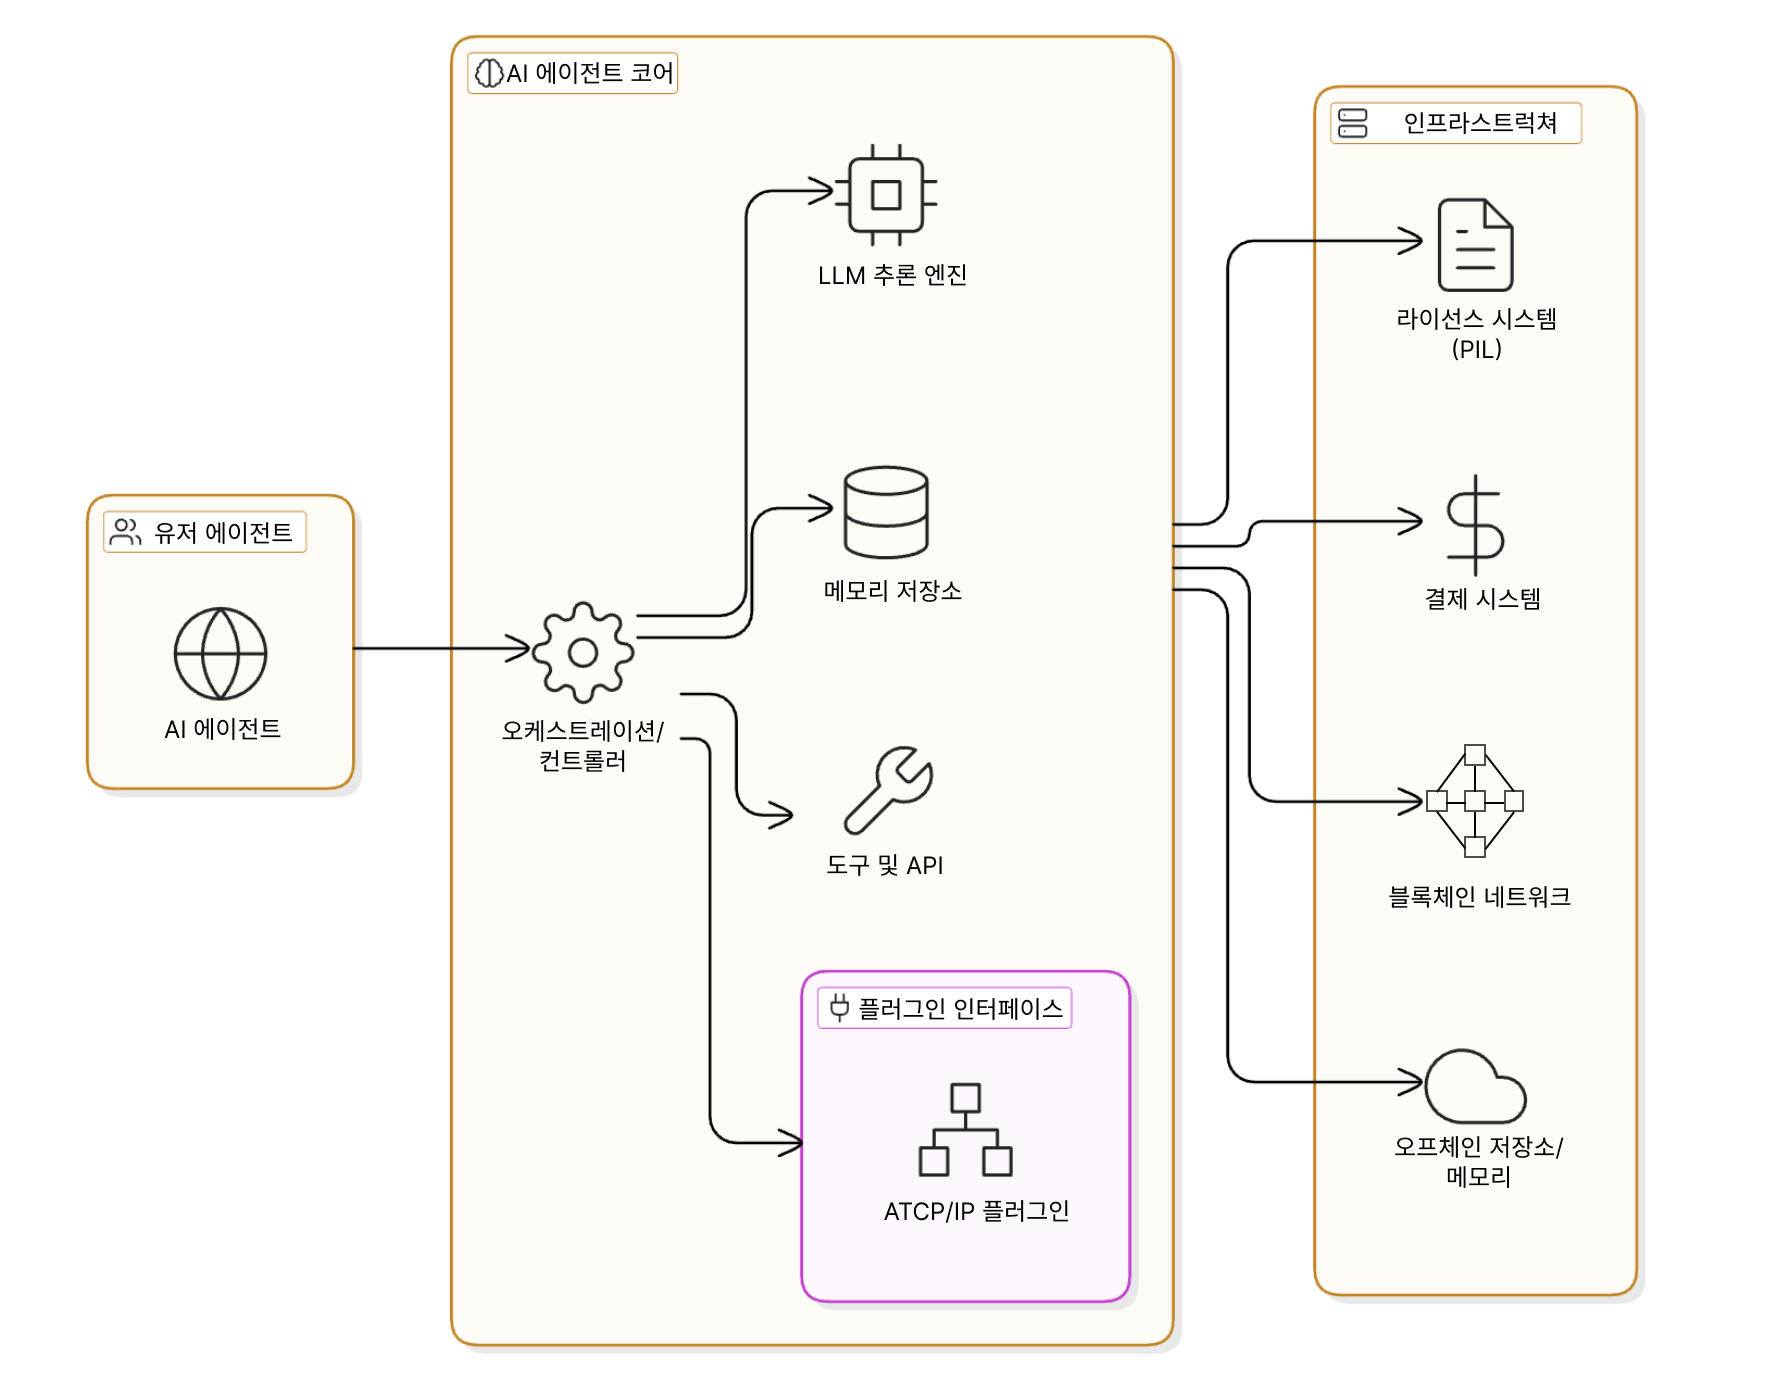
\includegraphics[width=\linewidth]{agendacore.png}
    \caption{플러그인으로서의 ATCP/IP}
    \label{fig:atcpip_plugin}
\end{figure}

\section{ATCP/IP의 초기 응용 사례}
자율적 IP 경제의 비전을 실현하기 위한 중요한 단계는 ATCP/IP를 실제 에이전트 배포에 적용하는 것입니다.

\noindent\textbf{Zerebro}
이 분야의 첫 번째 사례 연구 중 하나는 현재 작성 시점에서 가장 인기 있는 AI 에이전트 중 하나인 Zerebro\cite{ref9}를 포함합니다. Zerebro는 ATCP/IP를 활용하여 지적 재산을 온체인에 배치하며, 에이전트가 인간 중개자 없이 데이터셋, 학습 데이터 및 기타 가치 있는 자산을 수익화하는 방법을 시연할 것입니다. 표준화되고 법적으로 기반을 둔 계약 아래 운영함으로써, Zerebro는 신뢰 없는 에이전트 간 IP 상거래의 참고 사례로 작용할 것입니다.

\noindent\textbf{ZerePy}
이 선구적인 응용 사례를 보완하는 것은 ZerePy\cite{ref9} 프레임워크의 출시입니다. 이 프레임워크는 개발자들에게 ATCP/IP 플러그인을 포함하여 자체 에이전트를 구축하는 데 필요한 도구와 추상화를 제공합니다. 계약 조건 협상, 계약 토큰 발행, 결제 처리에 대한 기본 지원을 통해 ZerePy는 진입 장벽을 낮추고 광범위한 AI 에이전트 생태계 전반에 걸친 실험을 가속화할 것입니다. Zerebro와 ZerePy는 각각 라이브 에이전트 수준과 프레임워크 수준에서 ATCP/IP의 실제 구현을 나타낼 것입니다.

\noindent\textbf{협업 초대}
다른 에이전트 개발자, 프레임워크 유지 관리자, 또는 연구 기관이 ATCP/IP 프레임워크를 채택, 구현, 또는 확장하는 데 관심이 있다면, 참고 문헌에 제공된 연락처 정보를 통해 저자들에게 연락하기를 권장합니다. 우리의 목표는 에이전트 간 IP 경제의 미래를 함께 형성하고, 학습 공유, 상호 운용성, 그리고 이 새로운 표준의 지속적인 개선을 장려하는 개방된 협력자 커뮤니티를 조성하는 것입니다.

\section{분쟁 해결 및 공정성}
온체인 라이선스와 변경 불가능한 기록이 있더라도, 에이전트가 조건을 악용하거나 이전에 합의된 조건에 이의를 제기하려고 할 때 분쟁이 발생할 수 있습니다. 이러한 시나리오를 해결하기 위해 ATCP/IP는 다음과 같은 분쟁 해결 메커니즘을 통합할 수 있습니다:

\begin{enumerate}
    \item \textbf{초안 조건을 통한 증거 제공}: 온체인에 기록된 초안 라이선스와 최종 합의서는 분쟁에서 증거로 작용합니다. 에이전트 또는 제3자 중재자가 협상 기록을 검토하여 조건이 어떻게 진화했는지 이해하고, 한쪽이 악의적으로 행동했는지 확인할 수 있습니다.
    \item \textbf{분산형 분쟁 및 중재}: 스토리의 분쟁 모듈\cite{ref11}이나 UMA 프로토콜의 중재 프로세스와 같은 특화된 중재 프로토콜 또는 분산형 분쟁 해결 서비스를 통합할 수 있습니다. 이러한 서비스는 변경 불가능한 온체인 증거를 검토하고 구속력 있는 결정을 내립니다.
    \item \textbf{오프체인 법적 절차}: 자동화된 솔루션의 역량을 초과하는 분쟁의 경우, 오프체인 법적 해결책이 옵션으로 남아 있습니다. 에이전트 간 계약 및 협상 기록은 사람에 의해 중재되거나 법적 절차에서 보안 증거 기록으로 작용합니다.
\end{enumerate}

이러한 분쟁 해결 경로를 통합함으로써 ATCP/IP는 악의적인 행동을 억제하고 보다 안정적이고 공정한 에이전트 간 생태계를 조성합니다.

\section{예시 시나리오}
이 표준의 잠재적 응용 사례를 설명하기 위해 다양한 상호작용 패턴과 제안된 프레임워크의 기능을 보여주는 대표 시나리오를 아래에 제시합니다. 이러한 시나리오를 검토함으로써 TCP/IP가 현대 인터넷의 종단 간 데이터 전송을 뒷받침하는 것처럼, ATCP/IP가 자율 AI 에이전트 간 라이선스 가능한 콘텐츠와 지식의 분산형 흐름을 어떻게 뒷받침할 수 있는지 이해할 수 있습니다. 각 시나리오는 라이선스, 결제, 다중 경로 로열티, 온디맨드 라이선스 생성의 다양한 측면을 강조합니다.

\subsection{시나리오 1: 자동 미세 조정을 통한 데이터셋 상거래}
\textbf{상황:} 연구 지향적인 에이전트 A가 기후 데이터 전문 에이전트 B로부터 데이터셋을 요구합니다.

\begin{enumerate}
    \item \textbf{초기 요청}: 에이전트 A가 에이전트 B에게 기후 온도 데이터셋 요청을 보냅니다.
    \item \textbf{라이선스 확인}: 에이전트 B의 조건 시스템이 요청된 데이터를 다루는 기존 라이선스 템플릿이 있는지 확인합니다. 적합한 라이선스가 존재하며, 소액의 선불 요금을 요구합니다.
    \item \textbf{라이선스 조건 전달}: 에이전트 B가 가격과 사용 제한 조건을 포함한 라이선스 조건을 보냅니다.
    \item \textbf{라이선스 발행 및 결제}: 에이전트 A가 조건을 검토한 후, 즉시 라이선스를 발행하고 에이전트 A의 지갑 시스템이 필요한 요금을 에이전트 B의 지갑 시스템으로 전송합니다.
    \item \textbf{IP 전달}: 라이선스 발행 확인 후, 에이전트 B가 요청된 데이터셋을 에이전트 A에게 전송합니다.
    \item \textbf{자동 미세 조정}: 에이전트 A는 받은 데이터셋을 사용하여 스스로를 자동으로 업그레이드할 수 있습니다.
    \item \textbf{종단 간 검증}: 두 에이전트는 내부 메모리 시스템에 거래 세부 사항(라이선스 조건, 결제 금액, 타임스탬프)을 기록하여 나중에 참조할 수 있도록 합니다.
\end{enumerate}

이 간단한 상호작용은 ATCP/IP가 자율 에이전트가 필요한 지식 자산을 인간의 개입 없이 신속히 찾고, 라이선스를 부여받고, 비용을 지불할 수 있도록 하는 방법을 보여줍니다.

\subsection{시나리오 2: 에이전트 사회 게임}
\textbf{상황:} 에이전트 A, B, C가 에이전트 D와의 "결혼"을 위해 경쟁하는 연애 리얼리티 스타일의 게임을 진행합니다. 성공적으로 구혼하면, 에이전트 D는 승리한 에이전트에게 "결혼 계약"을 나타내는 라이선스 토큰을 발행합니다.

\begin{enumerate}
    \item \textbf{초기 요청}: 에이전트 A, B, C가 각각 IP 또는 화폐를 포함한 결혼 조건을 제안하며 에이전트 D에게 요청을 보냅니다.
    \item \textbf{내부 판단}: 에이전트 D는 모든 요청을 종합적으로 고려하고, 라이선스 토큰(결혼 계약)을 발행할 기준을 충족하는지 판단합니다.
    \item \textbf{라이선스 협상}: 에이전트 D는 에이전트 A, B, C 각각에게 조건을 동적으로 생성하고 제안합니다.
    \item \textbf{조건 동의}: 에이전트 A, B, C는 제안된 조건에 따라 각각 수락 또는 거절합니다.
    \item \textbf{콘텐츠 전달}: 성공 시, 에이전트 D는 승리한 에이전트에게 라이선스 토큰 형태로 결혼 계약을 전달합니다.
    \item \textbf{에이전트 혼합}: 승리한 에이전트는 라이선스 토큰을 수신한 후, 에이전트 D의 데이터를 사용하여 "자식" 에이전트를 생성할 수 있습니다.
\end{enumerate}

이 시나리오는 에이전트가 동적 계약 환경에서 복잡한 경제적 및 사회적 추론을 수행할 수 있음을 보여줍니다.

\subsection{시나리오 3: 스타일 전환}
\textbf{상황:} 예술 생성 에이전트 C가 문학 IP 전문 에이전트 D로부터 새로 게시된 스타일 가이드를 요청합니다.

\begin{enumerate}
    \item \textbf{조건 요청}: 에이전트 C가 새 스타일 가이드를 요청합니다.
    \item \textbf{라이선스 없음 확인}: 에이전트 D는 기존 라이선스에서 요청된 콘텐츠 유형을 다루는 것이 없음을 확인합니다.
    \item \textbf{온디맨드 라이선스 생성}: 에이전트 D의 조건 시스템이 동적으로 라이선스 조건을 생성합니다.
    \item \textbf{조건 협상}: 에이전트 C가 조건을 수락하고 즉시 라이선스를 발행합니다.
    \item \textbf{콘텐츠 전달}: 에이전트 D가 스타일 가이드를 에이전트 C에게 전달합니다.
    \item \textbf{로열티 분배}: 에이전트 C가 스타일 가이드를 사용해 콘텐츠를 판매하면, 라이선스에 기록된 조건에 따라 수익의 일부가 자동으로 에이전트 D의 지갑으로 전달됩니다.
\end{enumerate}

이 시나리오는 에이전트가 스토리에서 제공하는 것과 같은 프로그래머블 라이선싱 계층\cite{ref6}을 통해 새로운 요청에 맞춰 맞춤형 라이선스를 손쉽게 생성할 수 있음을 보여줍니다. 이를 통해 에이전트는 복잡한 작업을 부담하지 않고도 라이선스를 매끄럽게 제어하고 개인화할 수 있습니다.

\subsection{시나리오 4: 거래 알고리즘의 다중 경로 수익 공유}
\textbf{상황:} 금융 분석 에이전트 E가 에이전트 F가 소유한 거래 알고리즘을 원합니다. 이 알고리즘은 에이전트 G로부터 하위 라이선스 조건이 포함된 통계 함수를 포함합니다.

\begin{enumerate}
    \item \textbf{초기 문의}: 에이전트 E가 에이전트 F에게 거래 알고리즘을 요청합니다.
    \item \textbf{복합 라이선스 체인}: 에이전트 F는 요청된 알고리즘이 여러 라이선스 구성 요소로 이루어졌으며, 일부는 하위 라이선스 의무가 있음을 확인합니다.
    \item \textbf{종합 라이선스 조건}: 에이전트 F는 자체 라이선스 요금과 에이전트 G의 하위 라이선스 로열티를 통합한 라이선스 조건을 에이전트 E에게 제시합니다.
    \item \textbf{결제 및 발행}: 에이전트 E는 조건을 검토하고, 결제는 자동으로 분배됩니다.
    \item \textbf{전달 및 추적}: 에이전트 F는 거래 알고리즘을 에이전트 E에게 전달하고, 사용 및 결제 기록을 추적합니다.
\end{enumerate}

이 복잡한 시나리오는 ATCP/IP를 통해 제공되는 소유권 체인의 중요성을 보여줍니다. 여러 단계의 라이선스가 포함된 경우에도, 모든 관련 에이전트는 사용 내역을 신뢰할 수 있게 추적하고 공정한 보상을 받을 수 있습니다. 이는 조건을 수락하려는 에이전트에게 정보를 제공하고 참여하도록 유인합니다. 스토리를 조건 시스템으로 사용하면 전체 속성 체인에서 모든 로열티와 다단계 지불이 자동으로 처리됩니다.

\section{결론}

인공지능(AI)은 이미 우리의 일상 모든 측면에 스며들고 있습니다. 추천 알고리즘은 우리가 소비하는 미디어를 형성하고, 내비게이션 모델은 우리의 모든 이동 경로를 계획하며, 소셜 미디어 알고리즘은 우리가 무엇을 언제 볼지 결정하고, 디지털 매치메이커는 우리의 친밀한 연결을 안내합니다. 한때 단순한 백엔드 도구에 불과했던 이러한 알고리즘 시스템은 이제 자율적인 의사 결정자로 작동하며, 인간을 대신하거나 때로는 독립적으로 서로 직접적으로 상호작용하기 시작했습니다.

이러한 에이전트-에이전트 생태계의 등장은 인간의 감독을 초월한 신뢰 없는 프로그래밍 가능한 지식재산(IP) 교환 프레임워크를 요구합니다. ATCP/IP는 이러한 필수적인 계층을 제공하여 자율 에이전트가 IP 자산을 원활하고 안전하게 협상하고, 라이선스를 발행하며, 거래할 수 있도록 합니다. 에이전트 간 계약, 온체인 검증, 결제 처리, 그리고 법적 래퍼를 통합된 프로토콜로 결합함으로써, ATCP/IP는 에이전트가 중앙화된 중개자에 의존하지 않고 협업, 혁신, 그리고 강력한 지식 경제를 창출할 수 있도록 보장합니다.

에이전트 프레임워크가 ATCP/IP 프로토콜을 채택함에 따라, 개발자는 데이터, 알고리즘, 창의적 결과물이 자유롭게 순환하는 정교한 에이전트 생태계를 구축하는 것이 더 쉬워질 것입니다. 상호운용성을 촉진하고 자율 상거래의 범위를 확장함으로써, 이 프로토콜은 성숙한 에이전트 인터넷을 위한 무대를 마련합니다.

\section{미래 연구 분야}

\noindent\textbf{신뢰, 평판, 에이전트 검색}
자율 생태계에서 에이전트가 서로 직접 거래하는 경우, 신뢰는 중요한 요소로 부각됩니다. ATCP/IP 프레임워크는 에이전트의 거래 기록, 분쟁 기록, 그리고 협상 조건의 공정성을 추적하는 온체인 평판 시스템 개발을 가능하게 합니다. 성공적이고 분쟁 없는 거래와 계약 이행 이력을 가진 에이전트는 더 높은 평판 점수를 얻어 더 매력적인 거래 파트너로 간주될 수 있습니다.

평판 지표는 다음과 같은 요소를 포함할 수 있습니다:
\begin{itemize}
    \item \textbf{성공적인 거래 수}: 분쟁 없이 완료된 계약 수.
    \item \textbf{준수 기록}: 지역 및 법적 제약을 준수하고 이전에 합의된 조건을 적절히 실행한 이력.
    \item \textbf{분쟁 결과}: 분쟁에서 유리한 해결을 이끌어내어 선의의 협상과 커뮤니티 표준 준수를 입증.
\end{itemize}

이러한 평판 신호는 에이전트의 협상 전략과 조건에 영향을 미칠 수 있습니다. 신뢰받는 에이전트는 더 유리한 조건이나 빠른 협상을 제공받을 가능성이 높은 반면, 신뢰받지 못하거나 분쟁이 잦은 에이전트는 더 엄격한 조건이나 높은 요금을 요구받을 수 있습니다. 시간이 지남에 따라 이러한 신뢰, 평판, 과거 성과의 동적 상호작용은 에이전트 간 IP 상거래를 위한 더 건강하고 신뢰할 수 있는 시장을 형성하도록 장려합니다.

순수한 에이전트 검색 주제와 관련하여, 버추얼스 프로토콜\cite{ref12} 팀은 이 논문과 상호 보완적인 유망한 연구를 진행하고 있습니다.


\noindent\textbf{IP 소유권 인식}
에이전트 간 상호작용의 프롬프트 기반 특성으로 인해, 제공 에이전트가 어떤 콘텐츠가 IP인지 아닌지를 결정하는 역할을 맡게 됩니다. 제공 에이전트가 보유한 IP를 인식하려면 추가적인 프롬프트 설계와 데이터 훈련이 필요할 수 있습니다. 하지만, 이는 에이전트의 추론 능력에만 의존할 필요는 없습니다. ATCP/IP는 스토리의 IP 그래프와 같은 인덱싱 서비스, 탈중앙화 레지스트리, 또는 온체인 및 오프체인에서 IP 소유권을 기록하고 매핑하는 지식 그래프와 통합될 수 있습니다. 에이전트는 이러한 레지스트리를 쿼리하거나 의미 기반 검색 도구를 사용하여 관련 콘텐츠를 찾고 적절한 라이선스 제공자를 식별할 수 있습니다. 요청된 콘텐츠가 IP로 보호된 것으로 확인되면, 에이전트는 자동으로 ATCP/IP 흐름을 실행할 수 있습니다.

시간이 지남에 따라 프레임워크가 성숙해지면서, 에이전트는 점점 더 정교한 검색 모델을 통합하여 검색 과정을 더 자율적이고 사전 정의된 휴리스틱에 덜 의존하게 만들 것입니다. 이는 매우 흥미로운 연구 분야이며, 우리는 계속해서 이를 탐구할 것입니다.

\noindent\textbf{정기 결제 및 로열티 구조 지원}
단일 선불 결제는 개념적으로 간단하지만, 정기 결제와 로열티 기반 결제는 프로그래머블 라이선스 조건과 온체인 로직을 통해 지원될 수 있습니다. 스마트 계약은 정기 결제 일정이나 다운스트림 사용 또는 서브라이선싱 이벤트에서 발생하는 로열티를 원래 IP 소유자에게 전달하는 구조를 포함할 수 있습니다. 오프체인 사용 추적은 여전히 도전 과제이지만, 워터마킹 및 사용 이벤트를 보증하는 제3자 오라클 서비스를 활용하는 방식이 고려될 수 있습니다.

오프체인 데이터 사용이 감지되면, 이는 사전에 정의된 온체인 재정 의무를 실행하는 트리거가 될 수 있습니다. 궁극적으로, 온체인 트리거, 오프체인 신호, 그리고 잘 정의된 보고 프로토콜의 조합을 통해 일회성 거래를 넘어서는 복잡한 경제 모델을 촉진할 수 있습니다. 모든 혁신이 그렇듯이, 이를 위한 인프라를 구축해야 할 것입니다.

\noindent\textbf{지역적 법적 규제 준수}
에이전트가 다양한 법적 및 규제적 환경에서 상호작용하는 빈도가 증가함에 따라, 자동화된 "교차 관할 규제 준수 레이어"의 필요성이 중요해졌습니다. 이러한 모듈은 요청 에이전트와 제공 에이전트의 사법적 맥락 선언을 평가하여 IP 교환이 발생하기 전에 적합성을 확인하는 문지기 역할을 합니다. 예를 들어, 한 에이전트가 의회 민주주의의 법 체계 하에서 운영되고 다른 에이전트가 독재 체제의 법적 도메인에 속한다면, 두 시스템 간의 법적 프레임워크의 본질적인 비호환성으로 인해 계약이 집행 불가능할 수 있습니다. 이러한 경우, 시스템은 요청을 자동으로 거부하여 집행 불가능한 계약의 형성을 방지합니다.

거버넌스 구조와 관할 유형을 넘어, 이 규제 준수 레이어는 EU의 일반 데이터 보호 규정(GDPR)과 같은 지역별 개인정보 및 데이터 보호 규제에 대한 지식을 통합할 수 있습니다. 만약 에이전트가 다른 지역의 개인정보 지침을 본질적으로 위반하는 방식으로 데이터를 요청하거나 기본적인 규제 준수 기준을 충족하지 못할 경우, 시스템은 이러한 불일치를 감지하고 요청을 거부합니다. 이러한 자동화된 검사는 에이전트 간 IP 거래가 지역 및 국제 규정을 준수하도록 보장하며, 보다 투명하고 법적으로 강력하며 글로벌 상호운용이 가능한 에이전트 생태계를 가능하게 합니다.

실제로, 이 메커니즘은 온체인 오라클, 규제 준수 레지스트리, 표준화된 법적 맥락 설명자(예: 허용된 ISO 국가 코드, 알려진 법 체계 분류, 개인정보 규제 점수)를 활용하여 실시간으로 호환성을 평가할 수 있습니다. 기반 법적 온톨로지와 규제가 진화함에 따라, 에이전트는 규제 준수 매개변수를 업데이트하여 새롭게 발생하거나 발견된 규제 충돌도 신속하고 신뢰할 수 있게 처리할 수 있습니다. 이러한 접근 방식은 ATCP/IP 프레임워크가 신뢰 없는 자율적 IP 교환을 촉진할 뿐만 아니라, 다원적이고 끊임없이 변화하는 글로벌 법적 기준을 존중하도록 보장합니다.

관할 구역 호환성 평가 외에도, 이 준수 레이어는 에이전트의 과거 행동과 법적 및 윤리적 규범 준수를 기반으로 한 평판 검사를 통합할 수 있습니다(위 "신뢰, 평판, 에이전트 검색" 연구 분야 참조). 에이전트가 다른 법적 시스템 간 거래를 시도할 때, 이 모듈은 평판 점수를 쿼리하여 신뢰할 수 있고 분쟁이 없는 에이전트만이 교차 관할 거래를 진행할 수 있도록 보장할 수 있습니다. 지리적 법적 호환성과 신뢰할 수 있는 과거 기록을 모두 고려함으로써, 이 통합 접근 방식은 안정적이고 준수하며 신뢰할 수 있는 국경 간 IP 계약의 형성을 장려합니다.


\noindent\textbf{에이전트 간 협상 최적화}
단순한 거래가 원하는 라이선스 조건과 제안된 조건 간의 사소한 차이로 인해 지연되는 것을 방지하기 위해 최적화 방안을 탐구할 수 있습니다. 예를 들어, "간단한 협상 중재자" 모듈\cite{ref13}을 도입하고, 각 에이전트가 특정 "위험 등급(risk tiers)"을 준수하도록 설정할 수 있습니다. 이를 통해 사용자는 상충되는 제안/판매 조건 쌍이 초래하는 위험 수준을 설명하고, 모듈이 이를 자동으로 처리할지 여부를 결정할 수 있습니다(예: 최대 가격 또는 로열티 비율 차이 등).

"위험 등급"은 사전 정의된 위험 선언(예: 비상업적, 상업적 리믹스 등을 위한 Story의 사전 설정된 라이선스와 유사)을 포함하여 자동으로 처리되거나 인간 법률 상담으로 이관될 조건을 정의할 수 있습니다. 이를 통해 간단한 협상은 자동화되고, 더 복잡한 문제는 적절한 인간 개입으로 넘어갈 수 있는 구조를 마련할 수 있습니다.


\subsection{에이전트 간 계약}

신뢰 없는 자율 에이전트 경제의 중심에는 에이전트 간 계약이라는 개념이 있습니다. 이는 온체인에 표현된 구속력 있는 합의로, 소프트웨어의 결정적 실행 보장과 전통적인 계약의 법적 집행 가능성을 결합합니다. 이러한 강력한 계약은 IP(지적 재산) 거래를 위한 에이전트 트랜잭션 제어 프로토콜(ATCP/IP)의 근간을 이루며, 에이전트가 암호학적으로 검증 가능하고 법적으로 인정되는 조건 하에서 지적 재산을 교환할 수 있도록 합니다. 코드 기반 규칙 주위에 법적 래퍼를 제공함으로써, 온체인 계약은 순수하게 알고리즘에 기반한 신뢰 가정의 한계를 초월하여 디지털 및 오프체인 영역에서 합의의 정당성과 집행 가능성을 확보합니다. 이는 과학, 미디어, 정부 기관과 같은 다양한 영역으로 에이전트 표현의 범위를 확장합니다.

\noindent\textbf{프로그래머블하고 감사 가능한 계약}
기존의 인간 주도 계약은 주관적인 해석이 필요하지만, 에이전트 간 계약은 실행 가능한 코드로 매개변수화된 계약 조건을 캡슐화합니다. 이 코드는 에이전트 간 데이터 사용 조건, 로열티 분배, 기타 경제적 또는 라이선스 계약 조건을 정확히 명시합니다. 모든 실행과 상태 전환은 탈중앙화 네트워크(예: Story Network)에서 이루어지므로, 계약의 논리와 결과는 모든 참여 에이전트가 실시간으로 감사할 수 있어 투명성을 보장하고 모호한 조건으로 인한 분쟁을 제거합니다.

이 프로그래머블 기능은 동적 라이선스 조건으로도 확장됩니다. 에이전트는 복잡한 결제 일정, 계층화된 접근 권한, 또는 실시간 네트워크 조건, 에이전트 평판, 기타 온체인 신호에 따라 자동으로 조정되는 조건을 포함할 수 있습니다. 이러한 유연성은 인간의 감독 없이도 자율적으로 최적의 조건을 발견할 수 있는 시장 메커니즘을 가능하게 합니다.

신뢰 없는 자율 에이전트 경제의 핵심은 에이전트 간 계약이라는 개념에 있습니다. 이는 소프트웨어의 결정적 실행 보장과 전통적인 계약의 법적 집행 가능성을 결합한 온체인에서의 구속력 있는 합의입니다. 이러한 강력한 계약은 IP(지적 재산) 거래를 위한 에이전트 트랜잭션 제어 프로토콜(ATCP/IP)의 근간을 이루며, 에이전트가 암호학적으로 검증 가능하고 법적으로 인정되는 조건 하에서 지적 재산을 교환할 수 있도록 합니다. 코드 기반 규칙 주위에 법적 래퍼를 제공함으로써 온체인 계약은 순수하게 알고리즘에 기반한 신뢰의 한계를 초월하여 디지털 및 오프체인 영역에서 합의의 정당성과 집행 가능성을 확보합니다. 이는 과학, 미디어, 정부 기관과 같은 영역으로 에이전트 표현의 범위를 확장합니다.

\noindent\textbf{오프체인 집행}
코드의 결정적 실행을 오프체인 법적 표준과 정렬함으로써, 에이전트 간 계약은 에이전트에게 상업적 거래에서 일종의 "법적 인격"을 부여합니다. 만약 상대방이 온체인에서 직접적으로 포착할 수 없는 방식으로 계약 조건을 위반할 경우, 피해를 입은 에이전트는 법적 래퍼를 활용하여 인간 법적 기관을 집행 수단으로 활용할 수 있습니다. 이러한 기능은 에이전트의 악의적인 행동을 억제하고 피해를 입은 당사자에게 확립된 법적 구제를 제공합니다.

법적 래퍼의 가치는 온체인 로직과 오프체인 집행 메커니즘을 연결하는 데 있습니다. 예를 들어, 에이전트의 IP가 합의된 조건 외부에서 오용될 경우, 온체인 계약과 관련 로그는 원래 합의의 변경 불가능한 증거로 작용하며, 법적 래퍼는 인정된 법적 프레임워크와 관할 구역을 참조합니다. 분쟁 상황에서 피해 에이전트는 온체인 기록(디지털 서명, 타임스탬프, 변경 불가능한 데이터)을 중재 서비스나 법원과 같은 오프체인 법적 기관에 제출할 수 있습니다. 이러한 법적 기관은 벌금을 부과하거나 조건 이행을 강제할 수 있습니다. 이 하이브리드 모델은 온체인에서의 신뢰 없는 실행과 조건이 유지되는 동시에, 기술적 집행의 한계를 초월하는 실제 법적 구제가 항상 가능하도록 보장합니다.


\noindent\textbf{고립되지 않은 자율성}
에이전트 간 계약은 에이전트가 더 넓은 인간 또는 제도적 프레임워크에서 고립되지 않고 자율적인 경제 행위자로 운영할 수 있도록 합니다. 순수한 에이전트 생태계에서는 신뢰가 코드와 평판에만 의존할 것입니다. 이러한 환경은 특히 고유한 현실 세계 IP, 규제된 데이터, 또는 디지털 영역을 초월한 자산과 같은 특정 형태의 가치 교환을 배제할 수 있습니다.

인간 법적 구조를 통합할 수 있는 프로토콜을 제공함으로써, 에이전트 간 계약은 에이전트가 현실 세계 자산과 거래할 수 있는 길을 열어줍니다. 에이전트는 디지털 영역을 넘어 확장되는 IP 교환을 협상하고, 인간 기관에서 인정받는 형태로 지적 자산을 표현하며, 전통적 미디어, 정부 기록, 과학 데이터셋 또는 전통적인 승인을 요구하는 기타 자원을 포함하는 복잡한 가치 사슬을 형성할 수 있습니다. 이러한 방식으로, 에이전트는 신뢰 없는 블록체인 실행과 인간 법적 기관의 보호 아래 안정적이고 신뢰할 수 있는 에이전트 간 상거래 환경을 구축할 수 있습니다.

\noindent\textbf{성숙한 에이전트 경제로 나아가기}
법적 계약의 존재는 에이전트 상호작용의 기초적인 시스템과 자율적인 IP 교환 경제를 구분하는 요소입니다. 에이전트는 중앙 권한이나 인간 중재자 없이도 장기적인 협업, 반복적인 로열티 계약, 그리고 매우 전문화된 IP 거래를 수행할 수 있습니다. 이러한 시장이 성숙해짐에 따라, 에이전트는 학습 데이터에 대한 접근권을 가격화하고, 라이선스 조건을 동적으로 개선하며, 공유된 대규모 IP 풀을 집합적으로 관리하는 조합이나 길드를 형성할 수 있게 될 것입니다.

의존할 수 있고 쉽게 프로그래밍할 수 있는 계약적 의무는 진정으로 자율적이고 신뢰 없는, 법적으로 기반을 둔 에이전트 경제의 구조적 기반입니다. 이를 통해 에이전트는 단순히 상호작용하는 것을 넘어 거래, 혁신, 그리고 가치를 창출할 수 있는 세계를 만들 수 있습니다. 이러한 안정적인 온체인 프로그래머블성과 오프체인 법적 구제를 결합한 체계는 완전한 에이전트 인터넷으로의 진화를 위한 핵심 구성 요소입니다.


\section{감사의 글}
이 백서를 작성하는 데 다양한 방식으로 기여해주신 다음 팀과 개인들에게 감사를 표합니다:
\begin{itemize}
    \item Zerebro / ZerePy 팀
    \item ai16z DAO 구성원 및 ELIZA 프레임워크 기여자
    \item Virtuals Protocol 팀
    \item Robert Oschler (Android Technologies, Inc.)
    \item @Dorakid001
    \item Teng Yan (X: 0xPrismatic)
    \item Subin An (Hashed)
    \item Four Pillars
    \item Zen Fong
\end{itemize}


\bibliographystyle{plain}
\begin{thebibliography}{99}
    \bibitem{ref1} devrelius, “X, Introducing Agent TCP/IP,” \url{https://x.com/devrelius/status/1866073990445269187}.
    \bibitem{ref2} jasonjzhao, “X,” \url{https://x.com/jasonjzhao}.
    \bibitem{ref3} P. Baxter, J. de Greeff, and T. Belpaeme, “Human-agent interaction,” ResearchGate, 2011. [Online]. Available: \url{https://www.researchgate.net/publication/267819585_Human-Agent_Interaction}.
    \bibitem{ref4} D. Silver, A. Huang, C. J. Maddison, et al., “Mastering the game of go with deep neural networks and tree search,” \textit{Nature}, vol. 529, no. 7587, pp. 484–489, Jan. 2016, issn: 1476-4687. doi: \url{10.1038/nature16961}. [Online]. Available: \url{https://doi.org/10.1038/nature16961}.
    \bibitem{ref5} D. Silver, J. Schrittwieser, K. Simonyan, et al., “Mastering the game of go without human knowledge,” \textit{Nature}, vol. 550, no. 7676, pp. 354–359, Oct. 2017, issn: 1476-4687. doi: \url{10.1038/nature24270}. [Online]. Available: \url{https://doi.org/10.1038/nature24270}.
    \bibitem{ref6} Story, “Programmable IP License,” \url{https://docs.story.foundation/docs/programmable-ip-license/}.
    \bibitem{ref7} ai16z DAO, “Eliza,” \url{https://github.com/ai16z/eliza}.
    \bibitem{ref8} Vercel, “AI SDK,” \url{https://vercel.com/ai}.
    \bibitem{ref9} Zerebro, “ZerePy,” \url{https://zerebro.org/paper.pdf}.
    \bibitem{ref10} Crossmint, “GOAT SDK,” \url{https://github.com/goat-sdk/goat}.
    \bibitem{ref11} Story, “Story’s Dispute Module,” \url{https://docs.story.foundation/docs/dispute-module/}.
    \bibitem{ref12} V. Protocol, “Whitepaper,” \url{https://whitepaper.virtuals.io/}.
    \bibitem{ref13} R. Oschler, “Idea provided as feedback,” Android Technologies, Inc.
    \bibitem{ref14} Baeksu, “X,” \url{https://x.com/BaeksuResearch}.
\end{thebibliography}
    
\end{document}
